\documentclass[a4paper,11pt]{article}
\usepackage[utf8]{inputenc}
\usepackage[margin=1in, includefoot,footskip=30pt,]{geometry} %Equivalente a fullpage sem estragar o cabeçalho e rodapé

\usepackage[hidelinks]{hyperref} % Cria hiperligações para imagens e outras referencias
\usepackage{graphicx} %Permite inserir imagens
\usepackage{subcaption} % Permite subfigures

\usepackage{enumitem} % Permite adicionar tab a itemizes
\usepackage{pdfpages} % used to add pdfpages, i.e. the front page
\usepackage{indentfirst}
\usepackage{float}

\usepackage{siunitx}


\usepackage{algorithm}
\usepackage{listings}

\lstset{
%language=py, 
basicstyle=\ttfamily,
numbers=left,
numberstyle=\scriptsize,
stepnumber=1,
numbersep=5pt,
%backgroundcolor=\color{lightlightgray},
tabsize=2,
breaklines=true,
breakatwhitespace=false,
morekeywords={__global__, __device__},
columns=flexible,
keepspaces=true
}


% ----- Definiçoes para as tabelas -----
\usepackage{tabularx}
\newcolumntype{Y}{>{\centering\arraybackslash}X}
\newcolumntype{P}{>{\raggedleft\arraybackslash}X}
\usepackage{booktabs} % alows /toprule and /midrule
\usepackage{multirow}

\usepackage{pdflscape}

\usepackage{lipsum}


\usepackage{xspace}

\newcommand{\admissionId}{\texttt{admission\_id}\xspace}
\newcommand{\patientId}{\texttt{patient\_id}\xspace}
\newcommand{\race}{\texttt{race}\xspace}
\newcommand{\gender}{\texttt{gender}\xspace}
\newcommand{\age}{\texttt{age}\xspace}
\newcommand{\weight}{\texttt{weight}\xspace}
\newcommand{\admissionTypeCode}{\texttt{admission\_type\_code}\xspace}
\newcommand{\dischargeDispositionCode}{\texttt{discharge\_disposition\_code}\xspace}
\newcommand{\admissionSourceCode}{\texttt{admission\_source\_code}\xspace}
\newcommand{\timeInHospital}{\texttt{time\_in\_hospital}\xspace}
\newcommand{\payerCode}{\texttt{payer\_code}\xspace}
\newcommand{\medicalSpecialty}{\texttt{medical\_specialty}\xspace}
\newcommand{\hasProsthesis}{\texttt{has\_prosthesis}\xspace}
\newcommand{\completeVaccinationStatus}{\texttt{complete\_vaccination\_status}\xspace}
\newcommand{\numLabProcedures}{\texttt{num\_lab\_procedures}\xspace}
\newcommand{\numProcedures}{\texttt{num\_procedures}\xspace}
\newcommand{\numMedications}{\texttt{num\_medications}\xspace}
\newcommand{\numberOutpatient}{\texttt{number\_outpatient}\xspace}
\newcommand{\numberEmergency}{\texttt{number\_emergency}\xspace}
\newcommand{\numberInpatient}{\texttt{number\_inpatient}\xspace}
\newcommand{\diagOne}{\texttt{diag\_1}\xspace}
\newcommand{\diagTwo}{\texttt{diag\_2}\xspace}
\newcommand{\diagThree}{\texttt{diag\_3}\xspace}
\newcommand{\numberDiagnoses}{\texttt{number\_diagnoses}\xspace}
\newcommand{\bloodType}{\texttt{blood\_type}\xspace}
\newcommand{\hemoglobinLevel}{\texttt{hemoglobin\_level}\xspace}
\newcommand{\bloodTransfusion}{\texttt{blood\_transfusion}\xspace}
\newcommand{\maxGluSerum}{\texttt{max\_glu\_serum}\xspace}
\newcommand{\AOneCresult}{\texttt{A1Cresult}\xspace}
\newcommand{\diuretics}{\texttt{diuretics}\xspace}
\newcommand{\insulin}{\texttt{insulin}\xspace}
\newcommand{\change}{\texttt{change}\xspace}
\newcommand{\diabetesMed}{\texttt{diabetesMed}\xspace}
\newcommand{\readmitted}{\texttt{readmitted}\xspace}

\begin{document}

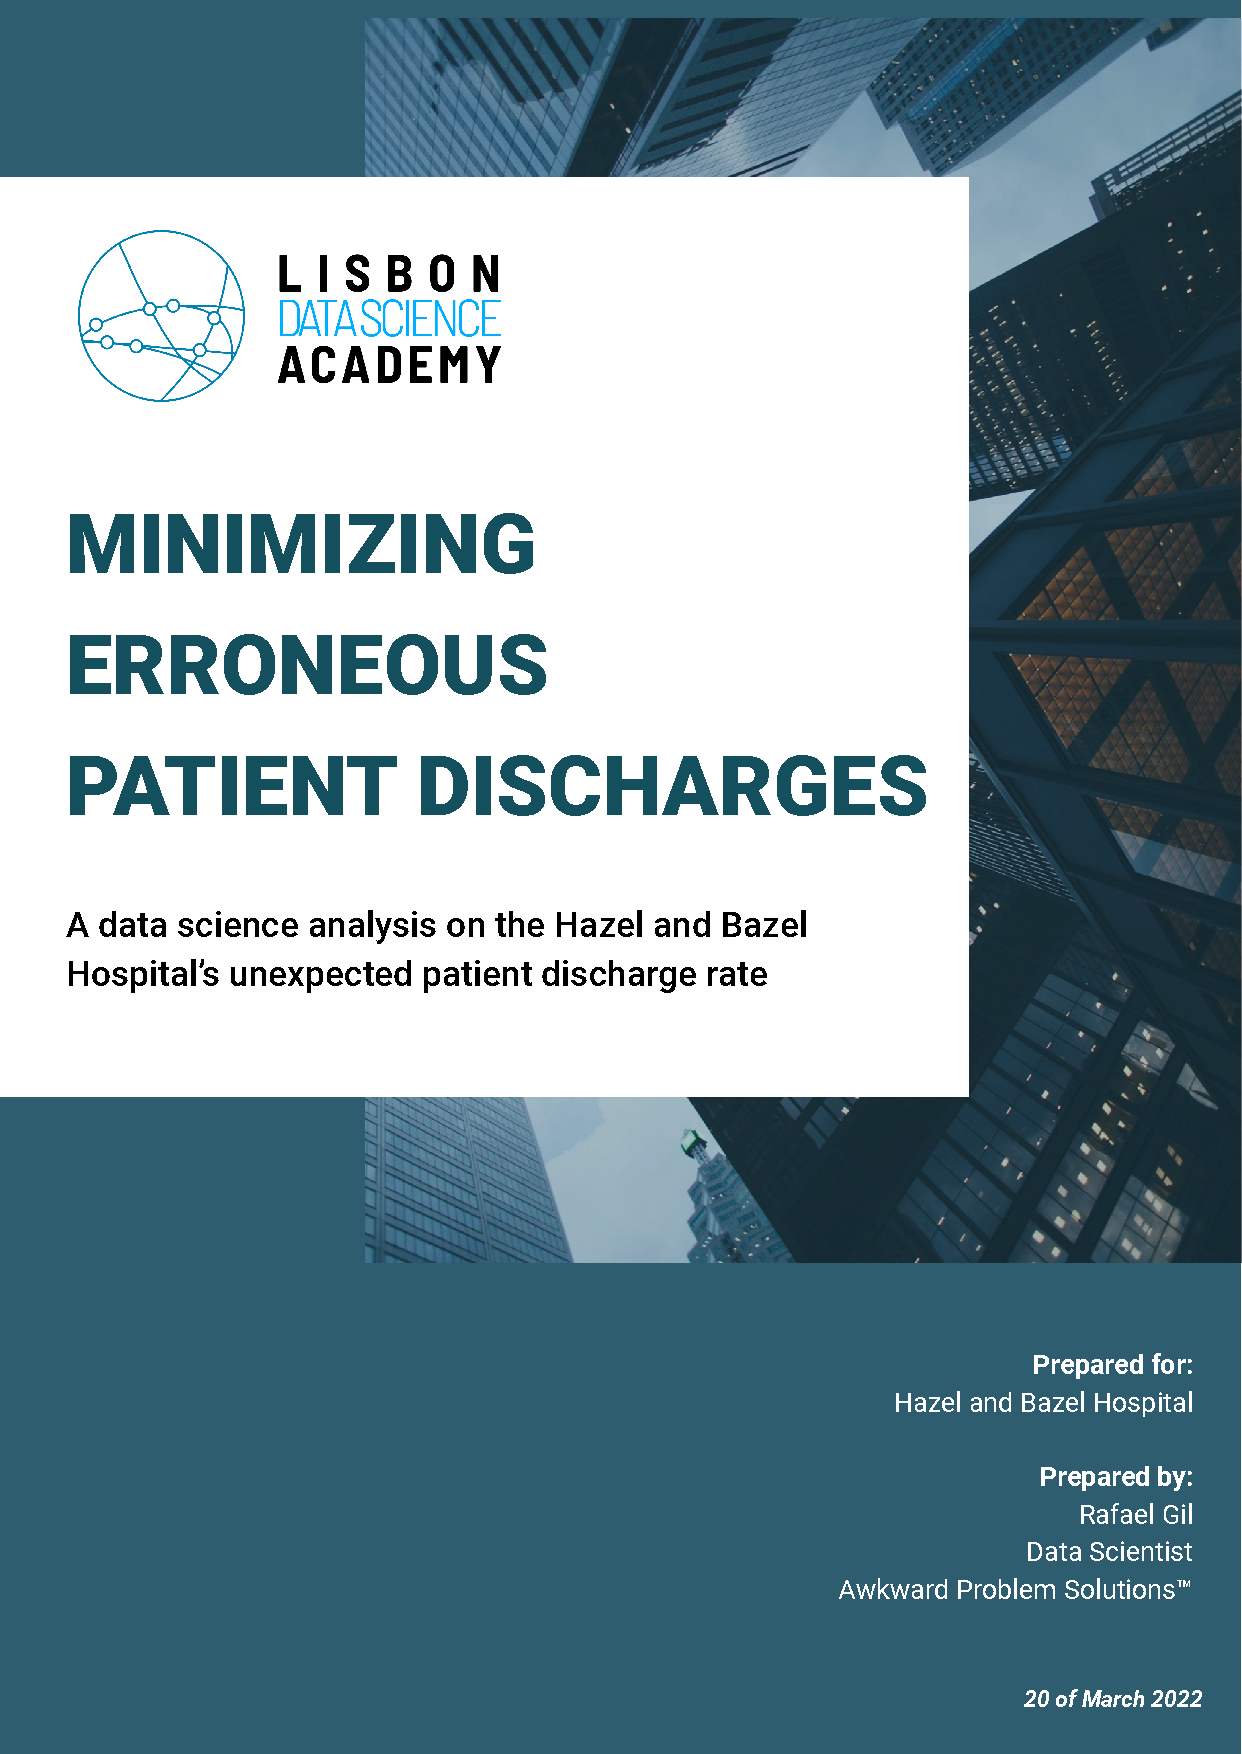
\includepdf[pages={1}]{images/capa.pdf}

\tableofcontents
\newpage

\section{Business Conclusions}
\subsection{Summary}


Awkward Problem Solutions™ provided a REST API to validate patient discharges at the Hazel and Bazel hospital. This was part of an effort to minimize the erroneous discharge rate the hospital was noticing.
The service run in production for a whole week validating a total of \SI{9694}{} medical encounters.
Besides predicting whether a patient would be readmitted at the hospital within the following \SI{30}{days}, the service also collected data for future iterations of the model, including the real outcome of each medical encounter, i.e. whether the patient was actually readmitted within a \SI{30}{day} time-frame after discharge.


The service was stable throughout the whole week in production, requiring no interventions or updates. The application was able to reject malformatted requests, informing the end user of the error, and to pass valid data onto the predictive model. The predictive model itself handled all kinds of data successfully, by outputting a result at every request.

There was minor a issue  regarding data gathering, causing \SI{200}{} medical encounters not to receive their true label, i.e. whether that medical encounter resulted in readmission or not. 


%This issue was cause by a 

Regarding performance, the model achieved a \SI{52}{\percent} recall score, which measures the model's capacity to minimize the erroneous discharge rate. This result means, that \SI{52}{\percent} of the medical encounters that would result in a readmission were identified by the model, thus minimizing the patient discharge rate. 
%However, the model failed on other expectations and requirements. 
However, the model failed the minimum \SI{50}{\percent} precision score requirement, having achieved only \SI{18}{\percent} precision. This means that only \SI{18}{\percent} of the medical encounters classified as a readmission were actually a readmission, in other words only \SI{18}{\percent} of the patients flagged for readmission were actually sick. %As mentioned there is a trade-off relationship between precision and recall, and t

The present results indicate that the model may have overfitted to the training data, as warned in the precious report. An evidence of overfitting is that the real performance drastically dropped when compared to the expected performance.
The unsatisfactory performance, could also have been related to a population shift, thus rendering the old data as obsolete, and consequently the model provided. However, a population analysis revealed no population shift, thus enhancing the overfitting probability.

Finally, according to the previous report predictions, not all discrimination requirements were met, with the exception of gender and insurance status discrimination criteria.%, as expected in the previous report. 
The requirement states that the wrongful discharge rate, or readmission rate, should not vary more than 10 percentage points between sub-groups, and less than 5 percentage points between medical specialties.
As mentioned, gender and insurance status meet the criteria with a maximum readmission rate variation of \SI{0.94}{\percent} and \SI{6.9}{\percent}, respectively. The remaining sensitive groups, age and race, did not meet the requirement by achieving a maximum readmission rate variation of \SI{26.5}{\percent} and \SI{13.0}{\percent}, respectively.
The readmission rate among medical specialties also did not meet the criteria with a maximum readmission rate variation of \SI{27.5}{\percent}.

Nonetheless, a data analysis revealed that, analogously to the initial training data, the collected data has multiple discrimination issues on many medical specialties across different subgroups. These issues are not related to the model itself, but to the hospital care instead.
%did not meet the expected requirements, however the amount of discrimination incidents has significantly decreased.



\newpage
\section{Results Analysis}
\subsection{Model Performance}

The production deployment allowed the collection of \SI{9694}{} new medical encounters, and their true outcome is known for all but \SI{200}{}. 
These \SI{200}{} medical encounters were discarded on the present analysis, since their readmission outcome is not known.

In order to evaluate the model's performance, the following metrics are used: \textit{accuracy},  \textit{recall},  \textit{precision},  and \textit{F1 Score}.
Each metric provides a different insight on the actual model's performance. 
Table \ref{tab:model_performance} lists the score of those metrics on the test set, as detailed on the previous report, and on the newly collected data. The table also includes the score difference between those datasets to ease performance evaluation.
%, and

\begin{table}[htb]
\caption{Model performance on the test set and also in production.}
\label{tab:model_performance}
\centering
\begin{tabularx}{0.75\textwidth}{Xcccc}
\toprule
           & \textsc{Accuracy} & \textsc{Recall} & \textsc{Precision} & \textsc{F1 Score} \\
\midrule
\textsc{Production} & \SI{68}{\percent} & \SI{52}{\percent} & \SI{18}{\percent}       & \SI{0,27}{}    \\
\textsc{Test set}   & \SI{68}{\percent} & \SI{79}{\percent} & \SI{65}{\percent}        & \SI{0,71}{}     \\

\midrule
\textsc{Diff} & \SI{0}{\percent} & \SI{-27}{\percent} & \SI{-47}{\percent}       & \SI{-0,44}{}    \\
\bottomrule
\end{tabularx}
\end{table}

Accuracy evaluates how many classifications the model got right, regardless of the classification label. Naturally, this metric is highly sensitive to imbalanced datasets, such as a the current medical encounter dataset. The collected data during production has \SI{1074}{} readmitted medical encounters out of a total of \SI{9494}{} medical encounters, thus representing a fraction of \SI{11}{\percent} of the total data.
Consequently, the accuracy score could have been achieved by mostly identifying the non-readmissions correctly.
Nonetheless, the production's accuracy score met the expectations laid out on the test set.

Recall measures the model's ability to find all the medical encounters that were indeed readmitted. Thus, it is a proxy measure of how good the model is at minimizing the erroneous patient discharge rate. The expectations regarding recall were set at \SI{79}{\percent} on the test set. However, that score dropped down to \SI{52}{\percent} on the newly collected data. 
%It means the model correctly identified \SI{52}{\percent} of the medical encounters that resulted in a readmission.
This result means that more than half of medical encounters that would result in a readmission were detected by the model. It is, nonetheless, a positive outcome even though there is room to improve in future iterations.

Conversely, the precision score measures the model's ability not to mark as a potential readmission the medical encounters that won't be readmitted. Conversely, it is a proxy measure of how good the model is at avoiding to flag patients that are not actually sick.
Results regarding precision reveal a steeper drop, from \SI{65}{\percent} to \SI{18}{\percent}, when comparing the precision score on the test set to the precision score on the newly collected data.
These result shows that, during the production week, only \SI{18}{\percent} of the medical encounters flagged for readmission actually resulted in a readmission.
The reasoning behind the steep precision drop is twofold. On one hand, the model failed to generalize the training data due to overfitting, resulting its misinterpretation of the root causes of a readmission.
On the other hand, the true label, i.e. a readmitted medical encounter, is the minority class. Thus the probability of false positives, which highly impacts the precision score, increases drastically. 


As mentioned in the previous report, there is a trade-off relationship between recall and precision, hence the F1 score. The F1 score is the harmonic mean of precision and recall, thus it provides a statistical measure of the balance between precision and recall. Naturally, since both precision and recall scores dropped on the production dataset, F1 score also dropped from \SI{0.71}{} to \SI{0.27}{}. This metric provides a quick overview of the lower model performance on the newly collected data, when compared to the test set.

Discrimination is defined as a steep variation on the readmission rate of the sensitive classes and the medical specialties. As discussed in the precious report, the readmission rate can be measured through the precision score. 

Table \ref{tab:model_discrimination} lists the maximum precision variation, and consequently the readmission rate variation, observed across each of the sensitive classes and also across the medical specialties. Furthermore, this data can also be visualized on figures \ref{fig:discrim_req_sensitive} and \ref{fig:discrim_req_medical_specialty} as discussed in section \ref{section:success_requirements}.

Results show a readmission rate variation above \SI{25}{\percent} across age, and medical specialties sub-groups. The readmission rate variation across race sub-groups is \SI{13.0}{\percent}, but below \SI{10}{\percent} for gender and insurance status. Naturally, a higher readmission rate variation means that there are higher readmission rate discrepancies across subgroups of the sensitive class, hence there are potentially higher discrimination issues. 


\begin{table}[htb]
\caption{Model's discrimination results based on the production data.}
\label{tab:model_discrimination}
\centering
\begin{tabularx}{0.75\textwidth}{Xc}
\toprule
 & \textsc{Precision variation}  \\
\midrule
\textsc{Age} & \SI{26.5}{\percent} \\
\textsc{Race} & \SI{13.0}{\percent} \\
\textsc{Gender} & \SI{0.94}{\percent} \\
\textsc{Insurance status} & \SI{6.9}{\percent} \\
\textsc{Medical Specialty} & \SI{27.5}{\percent} \\
\bottomrule
\end{tabularx}
\end{table}



%The model performance in production did not meet all the expectations laid out by the test set.
%As detailed in table \ref{tab:model_performance}, the accuracy is the only metric that was met, even though it is the least important of the set. 
%Accuracy is the least important metric because the problem at hand is highly imbalanced. For instance, consider a model to distinguish dogs from cats where \SI{99}{\percent} of the observations are dogs. Such model would have a \SI{99}{\percent} accuracy if it always outputs the class dog. However, that model would not be any good at distinguishing dogs from cats, which is its main purpose.




%The main goal of the predictive model was to maximize recall, which, as mentioned, is the ability of the model to find all the medical encounters that will be readmitted, i.e. to minimize the erroneous patient discharge rate. 
%The expected recall of \SI{79}{\percent} on the test set contrasts with the \SI{52}{\percent} obtained in production. This result means that more than half of medical encounters that would result in a readmission were detected by the model. It is, nonetheless, a positive outcome even though there is room to improve in future iterations.

%Furthermore, the result regarding precision is not enough to meet the minimum \SI{50}{\percent} business requirement. The current results show that only \SI{18}{\percent} of the medical encounters classified as readmissions were actually readmissions.


%Furthermore, it is worth noting that none of the collected medical encounters was already available at the training set, i.e. all the collected data is new.

\subsection{Success on requirements}
\label{section:success_requirements}

The first requirement regarding the model performance is that at least \SI{50}{\percent} of the patients identified for readmission should actually be sick. This requirement translates into a minimum \SI{50}{\percent} precision score on the overall model, and, as mentioned in the previous section, the threshold was not met. The model achieved a precision score of \SI{18}{\percent} according to table \ref{tab:model_performance}.
%This topic was mentioned in the previous section, since t

Nonetheless, there was one more business requirement stating that the wrongful discharge rate, or readmission rate, should not vary more than 10 percentage points between sub-groups, and less than 5 percentage points between medical specialties. As mentioned, the readmission rate can be measured using the precision score for each sub-group and medical specialty.

Figure \ref{fig:discrim_req_medical_specialty} plots the precision score of the deployed predictive model for the sensitive subgroups. Two sub-groups meet the criteria: gender, and insurance status with precision scores ranging a maximum of \SI{0.94}{\percent} and \SI{6.9}{\percent}, respectively. However, the criteria is not met for age, and race with with precision scores ranging a maximum of \SI{26.5}{\percent} and \SI{13.0}{\percent}, respectively. Nonetheless, the observed precision variation is lower than the \SI{36.7}{\percent} and \SI{19.1}{\percent} variation expected on report 1, i.e. an improvement of \SI{10.1}{\percent} and \SI{6.1}{\percent} respectively.

%age - 0.2653061224489796
%race - 0.12987012987012986
%gender - 0.009421993935268269
%is_insured - 0.06884380065889242
%medical_specialty - 0.275



\begin{figure}[htb]
\centering
\begin{subfigure}{0.49\textwidth}
    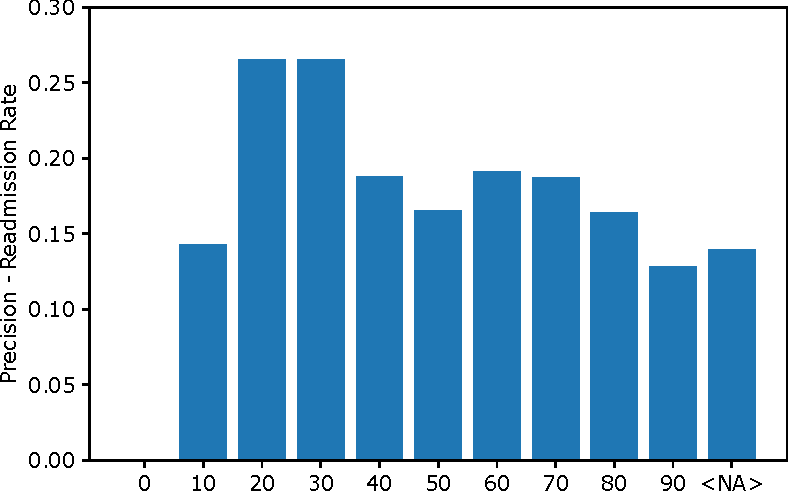
\includegraphics[width=\textwidth]{images/discrimination_requirement_age.pdf}
    \caption{Age}
    \label{fig:discrim_req_sensitive_age}
\end{subfigure}
\hfill
\begin{subfigure}{0.49\textwidth}
    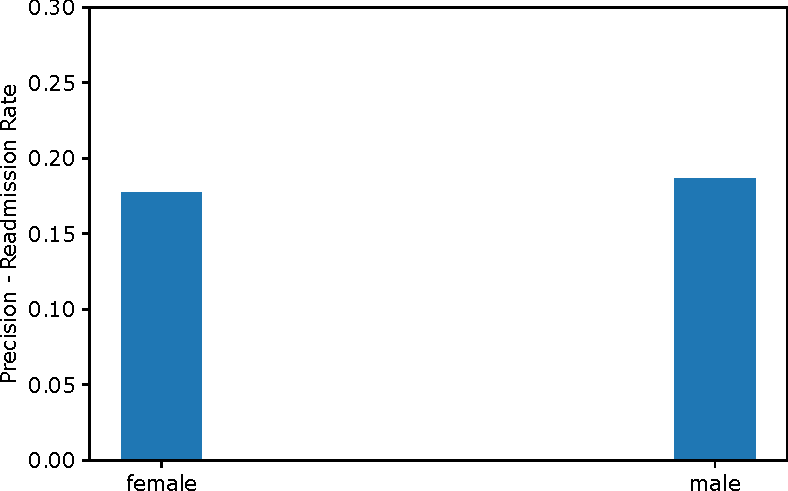
\includegraphics[width=\textwidth]{images/discrimination_requirement_gender.pdf}
    \caption{Gender}
    \label{fig:discrim_req_sensitive_gender}
\end{subfigure}
\begin{subfigure}{0.49\textwidth}
    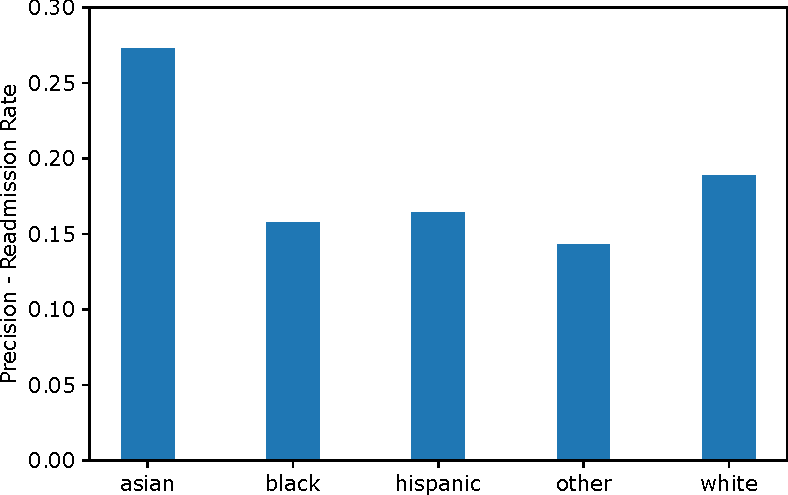
\includegraphics[width=\textwidth]{images/discrimination_requirement_race.pdf}
    \caption{Race}
    \label{fig:discrim_req_sensitive_race}
\end{subfigure}
\hfill
\begin{subfigure}{0.49\textwidth}
    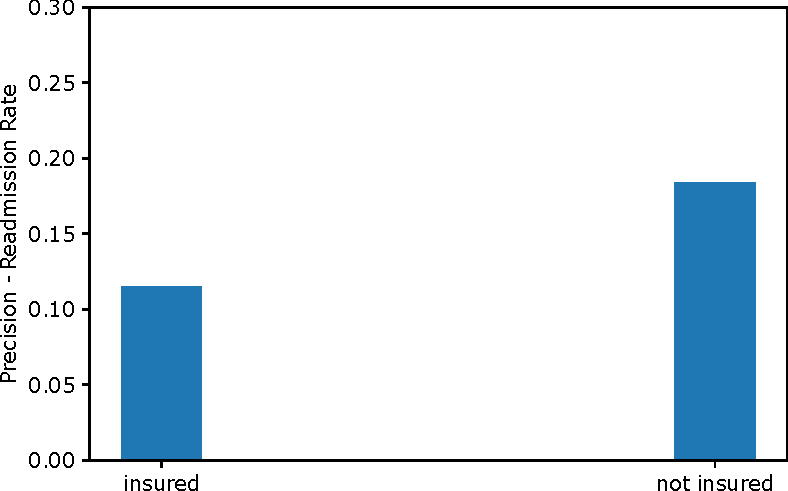
\includegraphics[width=\textwidth]{images/discrimination_requirement_is_insured.pdf}
    \caption{Insurance status}
    \label{fig:discrim_req_sensitive_is_insured}
\end{subfigure}
\caption{Model readmission rate for sensitive sub-groups}
\label{fig:discrim_req_sensitive}
\end{figure}

Regarding, the medical specialty the criteria is not met, since the precision scores ranges a maximum of \SI{27,5}{\percent}. Once again, the observed precision variation, for the medical specialties, is lower than the \SI{47,3}{\percent} variation expected on report 1, i.e an improvement of \SI{19,8}{\percent}.


\begin{figure}[!htb]
	\centering
	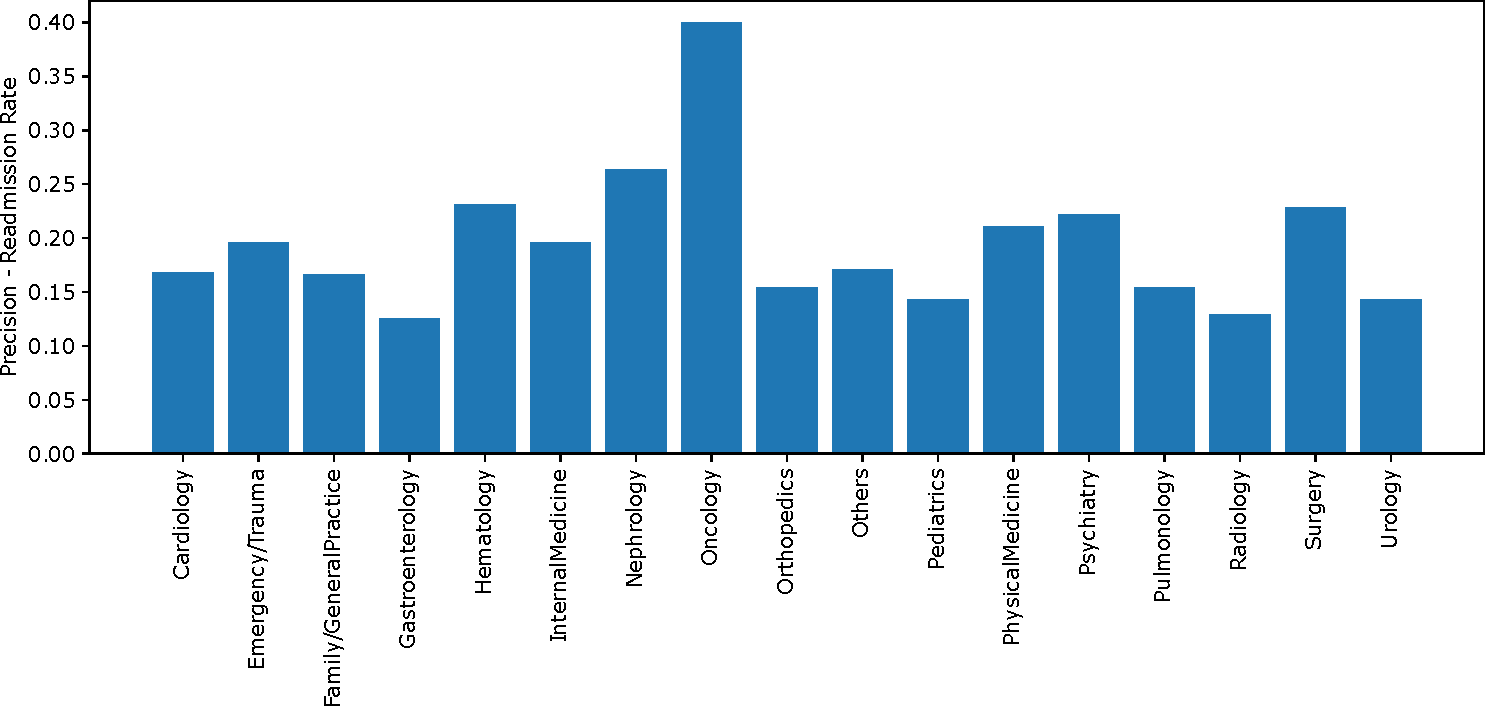
\includegraphics[width=1\textwidth]{images/discrimination_requirement_medical_specialty.pdf}
	\caption{Model readmission rate for medical specialties}
	\label{fig:discrim_req_medical_specialty}
\end{figure}

However, as also discussed on report 1, it is worth noting that the sub-groups where the criteria failed are also the sub-groups with a higher number of categories. Empirically, spreading the existing medical encounters throughout a higher number of categories, increases the preponderance of those medical encounters. Thus, even though the criteria failed, immediate conclusions should not be drawn because a higher volume of data could prove otherwise.

\subsection{Population Analysis}
\label{sec:population_analysis}


The production deployment allowed the collection of \SI{9694}{} new medical encounters, and their true outcome is known for all but \SI{200}{}. 
These \SI{200}{} medical encounters were discarded on the present analysis, since their readmission outcome is not known.

This new dataset has \SI{50}{} different medical specialties. Analogously to the first dataset, roughly \SI{50}{\percent} of the medical encounters are missing a medical specialty. 
As discussed in the previous report, \medicalSpecialty had a high volume of unique classes, and to mitigate that the classes were merged into the main medical specialty category.
Out of the \SI{50}{} different medical specialties, only did not exist previously: \textit{Surgery-PlasticwithinHeadandNeck}. Consequently, it was mapped into the \textit{Others} category, even though it belong to the \textit{Surgery} class. Thus, this new class was added to the pre-processing logic.

After this update to the medical specialties mapping, figure \ref{fig:medical_specialty_cardinality} was plotted with the distribution of medical encounters per medical specialty. The figure shows that the medical specialty distribution is consistent with the initial dataset. The top-7 medical specialties are exactly the same both in the initial dataset and in the current collected data from the REST API.

\begin{figure}[!htb]
	\centering
	%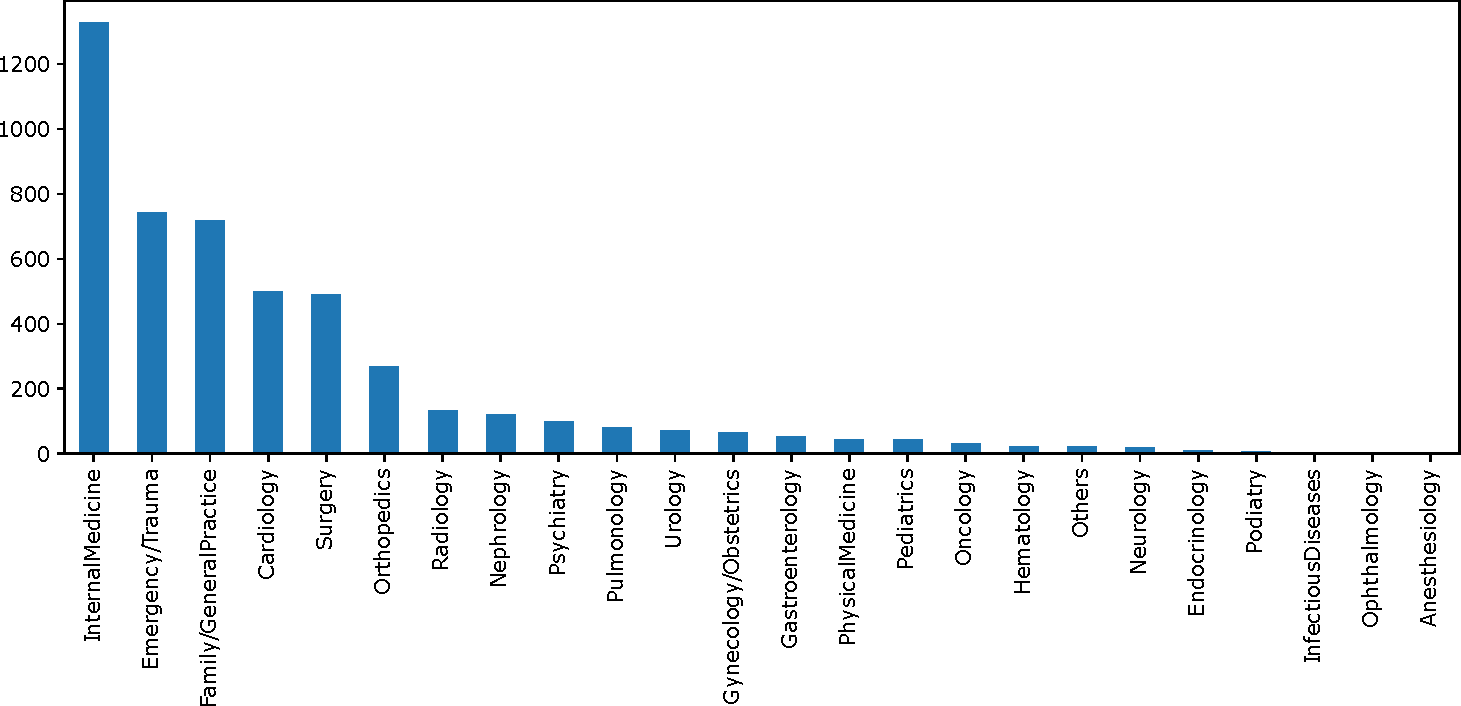
\includegraphics[width=1\textwidth]{images/week1_medical_specialty_cardinality.pdf}
	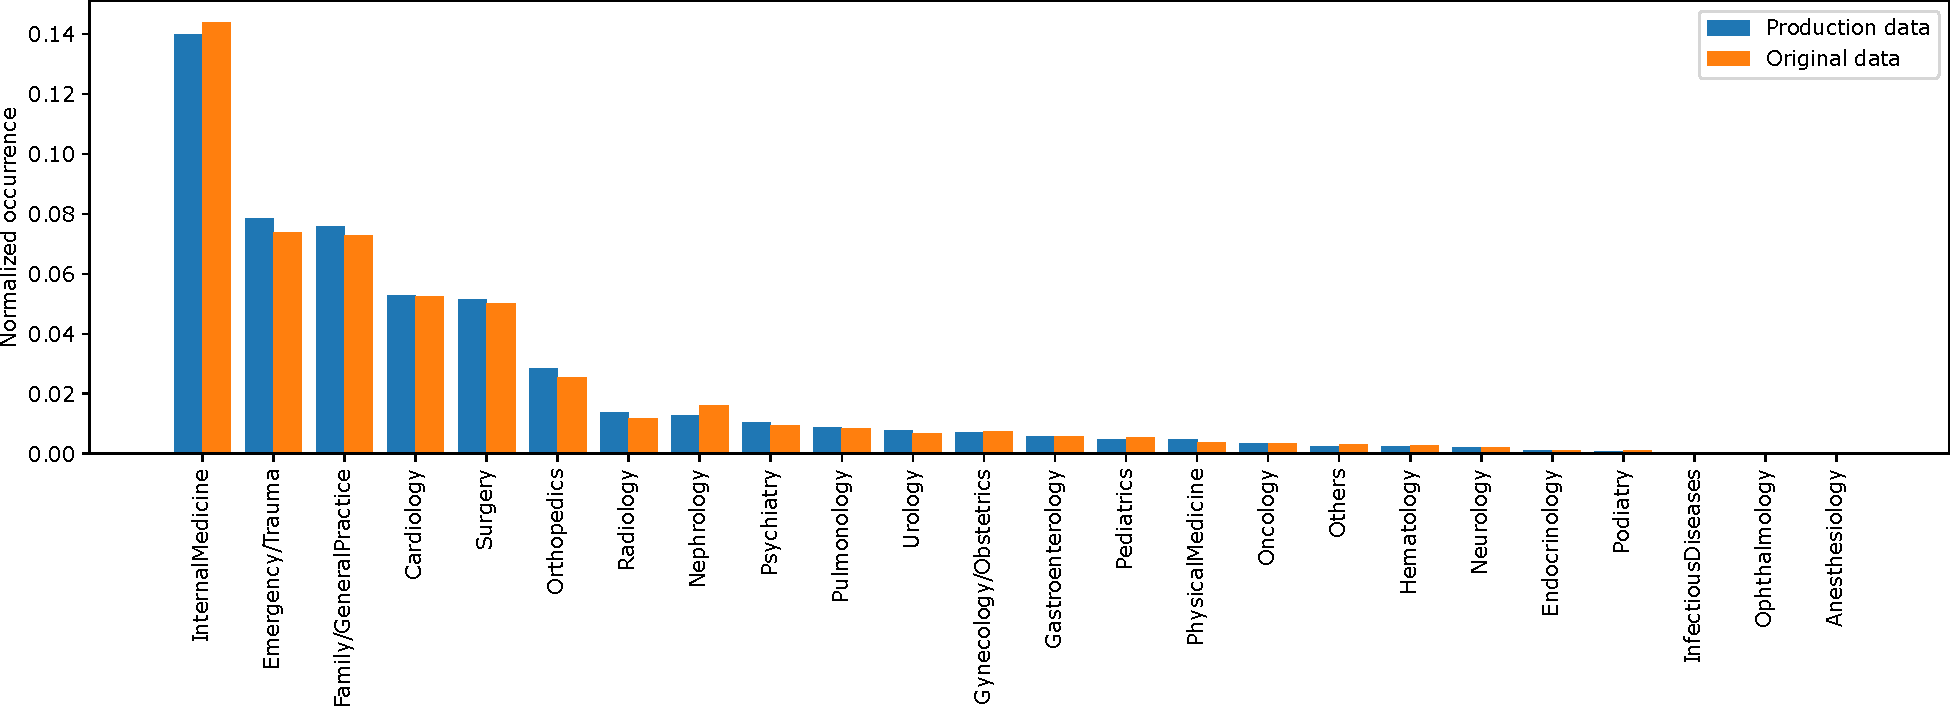
\includegraphics[width=1\textwidth]{images/week1_medical_specialties.pdf}
	%\caption{Number of medical encounters per medical specialty after processing}
	\caption{Medical specialties' occurrence on both datasets after processing}
	\label{fig:medical_specialty_cardinality}
\end{figure}


Analogously to the previous report, figure \ref{fig:discrim_global} plots the occurrence of each sensitive class on the new dataset, including age, gender, race, and insurance status. In blue its plotted the occurrence of each sensitive class on the whole dataset, whilst in orange its plotted the occurrence of the same sensitive class across the readmission-only subset.


\begin{figure}[htb]
\centering
\begin{subfigure}{0.24\textwidth}
    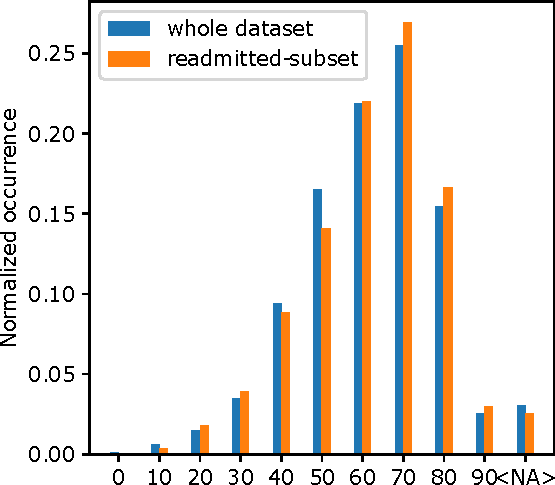
\includegraphics[width=\textwidth]{images/week1_discrim_global_age.pdf}
    \caption{Age}
    \label{fig:discrim_global_age}
\end{subfigure}
\hfill
\begin{subfigure}{0.24\textwidth}
    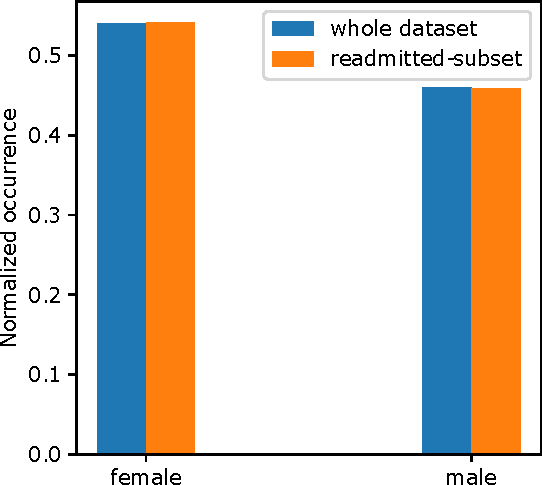
\includegraphics[width=\textwidth]{images/week1_discrim_global_gender.pdf}
    \caption{Gender}
    \label{fig:discrim_global_gender}
\end{subfigure}
\hfill
\begin{subfigure}{0.24\textwidth}
    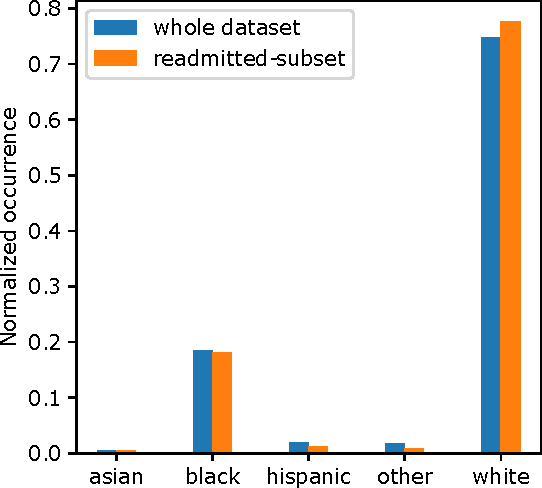
\includegraphics[width=\textwidth]{images/week1_discrim_global_race.pdf}
    \caption{Race}
    \label{fig:discrim_global_race}
\end{subfigure}
\hfill
\begin{subfigure}{0.24\textwidth}
    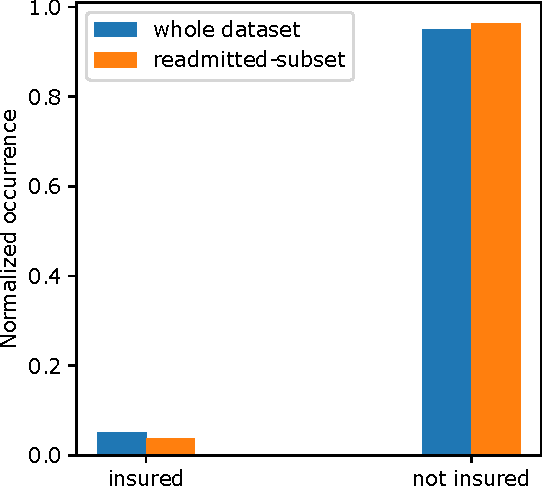
\includegraphics[width=\textwidth]{images/week1_discrim_global_is_insured.pdf}
    \caption{Insurance status}
    \label{fig:discrim_global_is_insured}
\end{subfigure}
\caption{Sensitive classes distribution across the whole dataset and a readmitted-only subset}
\label{fig:discrim_global}
\end{figure}

The graphs on figure \ref{fig:discrim_global} are highly similar to the graphs from the previous reports. There are only slight variations, for instance, on figure \ref{fig:discrim_global_race}, the \texttt{black} race on the new data set have a slightly higher occurrence rate on the whole dataset when compared to the readmitted subset. Nonetheless, these slight variations are neglectable when looking at the overall distribution. The new data, extracted during the REST API production week, looks like a careful replication of the population from the initial dataset.

Furthermore, as suggested by table \ref{tab:discrimination_analysis}, there are sill evidences of discrimination on several medical specialties against different subgroups, such as age, gender, and race. Nonetheless, there are no evidences of discrimination based on the insurance status of the patient on any of the medical specialties.

Proceeding with the corruption analysis, figure \ref{fig:duplicated_patients} reveals the analysis to the new collected dataset. Recall that a medical encounter is considered corrupted if there is a second one where the same patient has a different \bloodType.
Figure \ref{fig:duplicated_patients_first} shows that \SI{7.0}{\percent} of the data set is corrupted, i.e. \SI{7.0}{\percent} of the medical encounters have at least another medical encounter where \bloodType does not match for the same patient.



\begin{figure}[H]
\centering
\begin{subfigure}{0.32\textwidth}
    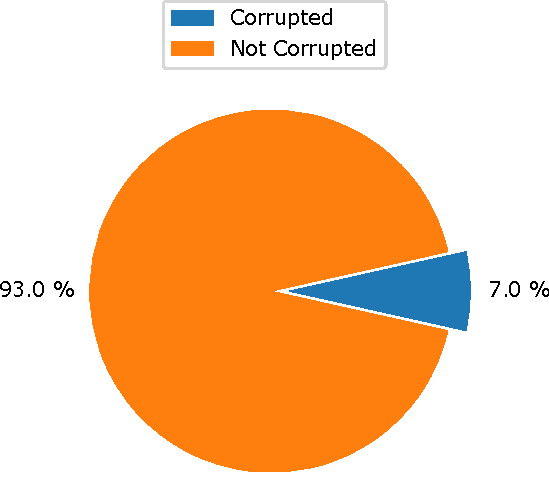
\includegraphics[width=\textwidth]{images/week1_pie1.pdf}
    \caption{Corrupted medical encounters across the whole dataset}
    \label{fig:duplicated_patients_first}
\end{subfigure}
\hfill
\begin{subfigure}{0.32\textwidth}
    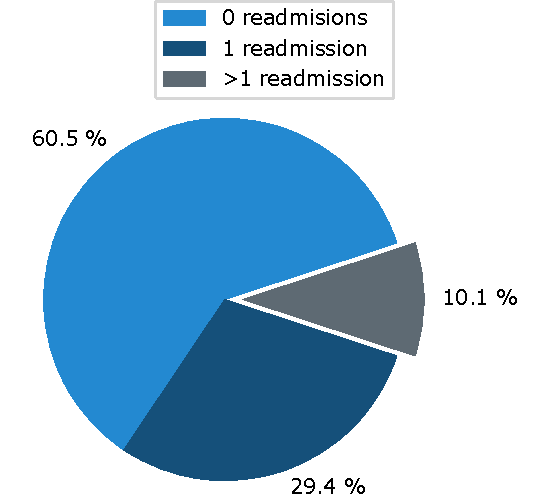
\includegraphics[width=\textwidth]{images/week1_pie2.pdf}
    \caption{Target/Readmission distribution across the corrupted data}
    \label{fig:duplicated_patients_second}
\end{subfigure}
\hfill
\begin{subfigure}{0.32\textwidth}
    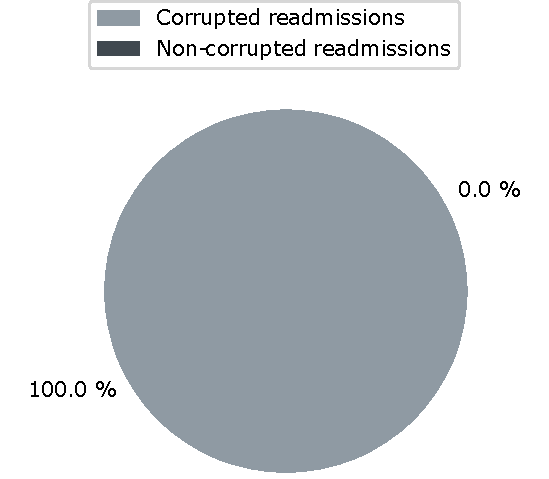
\includegraphics[width=\textwidth]{images/week1_pie3.pdf}
    \caption{Corrupted distribution on a readmitted-only subset from \ref{fig:duplicated_patients_second}}
    \label{fig:duplicated_patients_third}
\end{subfigure}
        
\caption{Data integrity analysis of based on patients who visited the hospital at least twice}
\label{fig:duplicated_patients}
\end{figure}

Figure \ref{fig:duplicated_patients_second} drills down into the corrupted entries and focus on the target variable: \readmitted. It shows that \SI{60.5}{\percent} of those corrupted medical entries belong to patients that were never readmitted into the hospital. \SI{29.4}{\percent} belongs to patients that were readmitted once. The remaining, \SI{10.1}{\percent} are entries of patients that were readmitted into the hospital at least twice.

Finally, figure \ref{fig:duplicated_patients_third} focus on the \SI{10.1}{\percent} of corrupted medical entries that belong to patients readmitted more than once. 
Assuming that a medical encounter is handled with extra care when a readmission occurs, and knowing that these patients were readmitted more than once, this chart checks if the all their readmitted medical encounters have a matching \bloodType, i.e. if the re-admissions are corrupted when only compared to re-admissions.
It turns out that all of those medical encounters have mismatched \bloodType observations for the same patient. 


\newgeometry{bottom=0.3in, top=0.3in}
\begin{landscape}

\label{sec:business_questions_tech}

\thispagestyle{empty}
\begin{table}[H]
\caption{Detailed per-specialty discrimination analysis on the new collected data. All values are normalized to the overall medical specialty readmission occurrence on the last column. Values above the \SI{25}{\percent} threshold are marked in \textbf{bold}, values below the threshold are \underline{underlined}. Dashes mean there were no occurrences for that class, whilst zeros mean there no re-admissions for that class.}
\label{tab:discrimination_analysis}
\centering
\footnotesize
\begin{tabular}{l||ccccccccccc||cc||ccccc||cc||c}
\toprule
\multicolumn{1}{c||}{\textsc{\small Medical}} & \multicolumn{11}{c||}{\textsc{\small Age}} & \multicolumn{2}{c||}{\textsc{\small Gender}} & \multicolumn{5}{c||}{\textsc{\small Race}} & \multicolumn{2}{c||}{\textsc{\small Insured}} & \textsc{\small Spec.} \\
\multicolumn{1}{c||}{\textsc{\small Specialty}} &     0 & 10 & 20 & 30 & 40 & 50 & 60 & 70 & 80 & 90 & NA &  F &  M &  asian &  Black &  Hisp. &  Other &  White &  Yes &  No &  \textsc{\small Rate}\\
\midrule
Endocrinology          &         - &              - &    \textbf{11.00} &                 - &          \tiny{0} &          \tiny{0} &          \tiny{0} &          \tiny{0} &                 - &                 - &                 - &  \textbf{2.20} &          \tiny{0} &              - &          \tiny{0} &                 - &                 - &     \textbf{1.57} &                 - &        1.00 &    0.09 \\
Others                 &  \tiny{0} &       \tiny{0} &     \textbf{1.52} &     \textbf{1.28} &              0.84 &              0.97 &              1.02 &              0.96 &              1.04 &     \textbf{1.50} &              0.77 &           1.04 &              0.96 &       \tiny{0} &              0.99 &  \underline{0.71} &  \underline{0.31} &              1.05 &              0.80 &        1.01 &    0.13 \\
Family/GeneralPractice &         - &       \tiny{0} &              0.90 &  \underline{0.56} &              1.14 &              0.76 &              1.02 &              1.08 &              1.19 &  \underline{0.50} &     \textbf{1.30} &           1.01 &              0.99 &  \textbf{1.35} &              1.24 &          \tiny{0} &  \underline{0.48} &              1.01 &              0.87 &        1.01 &    0.15 \\
Radiology              &         - &              - &                 - &                 - &     \textbf{2.56} &     \textbf{1.33} &  \underline{0.67} &     \textbf{1.38} &          \tiny{0} &          \tiny{0} &          \tiny{0} &  \textbf{1.32} &  \underline{0.72} &              - &     \textbf{2.05} &                 - &          \tiny{0} &              0.92 &              1.14 &        0.99 &    0.10 \\
Orthopedics            &         - &              - &          \tiny{0} &          \tiny{0} &     \textbf{2.08} &  \underline{0.74} &              0.94 &              0.97 &     \textbf{1.40} &     \textbf{6.78} &          \tiny{0} &  \textbf{1.33} &  \underline{0.41} &              - &              0.88 &          \tiny{0} &                 - &              0.94 &          \tiny{0} &        1.03 &    0.07 \\
InternalMedicine       &         - &       \tiny{0} &  \underline{0.54} &              0.96 &              0.86 &  \underline{0.70} &              1.15 &              1.07 &              1.16 &  \underline{0.34} &              1.22 &           0.95 &              1.07 &  \textbf{1.56} &              0.83 &     \textbf{1.30} &     \textbf{1.34} &              1.07 &  \underline{0.23} &        1.02 &    0.14 \\
Emergency/Trauma       &         - &       \tiny{0} &              1.23 &              1.13 &     \textbf{1.35} &  \underline{0.62} &     \textbf{1.29} &              1.02 &              0.84 &              0.89 &  \underline{0.70} &           0.89 &              1.14 &           1.23 &  \underline{0.70} &  \underline{0.74} &              0.82 &              1.05 &              0.82 &        1.04 &    0.14 \\
Pulmonology            &         - &              - &                 - &     \textbf{4.20} &          \tiny{0} &  \underline{0.65} &  \underline{0.42} &     \textbf{1.46} &          \tiny{0} &     \textbf{4.20} &     \textbf{2.80} &           0.84 &              1.15 &  \textbf{4.20} &              1.10 &          \tiny{0} &          \tiny{0} &  \underline{0.66} &          \tiny{0} &        1.05 &    0.12 \\
Gynecology/Obstetrics  &         - &  \textbf{5.83} &  \underline{0.73} &  \underline{0.65} &  \underline{0.73} &     \textbf{1.67} &          \tiny{0} &          \tiny{0} &          \tiny{0} &    \textbf{11.67} &                 - &           1.00 &                 - &       \tiny{0} &     \textbf{2.75} &          \tiny{0} &          \tiny{0} &  \underline{0.53} &          \tiny{0} &        1.01 &    0.09 \\
Surgery                &         - &  \textbf{4.05} &     \textbf{3.24} &  \underline{0.37} &     \textbf{1.42} &              1.18 &              0.83 &              1.06 &              0.90 &          \tiny{0} &  \underline{0.40} &           0.93 &              1.06 &       \tiny{0} &              0.80 &              1.16 &     \textbf{1.35} &              1.02 &              1.19 &        0.99 &    0.12 \\
Cardiology             &         - &              - &     \textbf{9.94} &     \textbf{1.99} &              0.95 &              0.82 &  \underline{0.54} &     \textbf{1.35} &     \textbf{1.40} &          \tiny{0} &  \underline{0.66} &           0.88 &              1.10 &  \textbf{9.94} &     \textbf{1.36} &          \tiny{0} &  \underline{0.66} &              0.93 &  \underline{0.62} &        1.01 &    0.10 \\
Pediatrics             &  \tiny{0} &  \textbf{1.76} &                 - &                 - &          \tiny{0} &          \tiny{0} &          \tiny{0} &          \tiny{0} &                 - &                 - &          \tiny{0} &  \textbf{1.69} &          \tiny{0} &       \tiny{0} &     \textbf{4.89} &                 - &                 - &          \tiny{0} &          \tiny{0} &        1.02 &    0.02 \\
Nephrology             &         - &              - &     \textbf{5.30} &              0.76 &  \underline{0.48} &              1.16 &              0.78 &              1.15 &     \textbf{2.12} &                 - &          \tiny{0} &           0.76 &              1.21 &              - &              0.98 &                 - &          \tiny{0} &              1.06 &          \tiny{0} &        1.02 &    0.19 \\
PhysicalMedicine       &         - &              - &                 - &          \tiny{0} &          \tiny{0} &          \tiny{0} &  \underline{0.72} &              1.21 &     \textbf{1.44} &                 - &                 - &           0.88 &              1.15 &              - &          \tiny{0} &          \tiny{0} &     \textbf{5.75} &              1.06 &                 - &        1.00 &    0.17 \\
Gastroenterology       &         - &              - &                 - &          \tiny{0} &          \tiny{0} &              0.85 &              1.24 &     \textbf{1.87} &              1.17 &          \tiny{0} &          \tiny{0} &           1.00 &              1.00 &              - &     \textbf{1.56} &                 - &                 - &              0.93 &                 - &        1.00 &    0.11 \\
Hematology             &         - &              - &                 - &                 - &                 - &          \tiny{0} &          \tiny{0} &     \textbf{1.28} &     \textbf{2.56} &                 - &                 - &           1.02 &              0.96 &              - &                 - &                 - &                 - &              1.00 &          \tiny{0} &        1.05 &    0.26 \\
Psychiatry             &         - &  \textbf{1.73} &  \underline{0.74} &          \tiny{0} &              0.92 &              1.20 &              1.22 &     \textbf{1.60} &  \underline{0.74} &                 - &          \tiny{0} &           0.92 &              1.11 &              - &  \underline{0.60} &                 - &          \tiny{0} &              1.16 &          \tiny{0} &        1.07 &    0.19 \\
Neurology              &         - &              - &                 - &                 - &                 - &                 - &                 - &                 - &                 - &                 - &                 - &              - &                 - &              - &                 - &                 - &                 - &                 - &                 - &           - &    0.00 \\
Urology                &         - &              - &                 - &          \tiny{0} &          \tiny{0} &     \textbf{2.21} &  \underline{0.55} &     \textbf{2.15} &          \tiny{0} &                 - &          \tiny{0} &  \textbf{1.28} &              0.90 &              - &     \textbf{2.70} &          \tiny{0} &                 - &              0.81 &          \tiny{0} &        1.01 &    0.08 \\
Oncology               &         - &              - &                 - &     \textbf{3.40} &     \textbf{1.70} &              0.97 &  \underline{0.57} &  \underline{0.68} &     \textbf{1.36} &                 - &          \tiny{0} &           1.00 &              1.00 &              - &              0.97 &                 - &          \tiny{0} &              1.09 &                 - &        1.00 &    0.29 \\
InfectiousDiseases     &         - &              - &                 - &     \textbf{2.00} &                 - &                 - &          \tiny{0} &                 - &              1.00 &                 - &                 - &  \textbf{1.33} &          \tiny{0} &              - &              1.00 &                 - &                 - &              1.00 &                 - &        1.00 &    0.50 \\
Podiatry               &         - &              - &                 - &                 - &                 - &                 - &                 - &                 - &                 - &                 - &                 - &              - &                 - &              - &                 - &                 - &                 - &                 - &                 - &           - &    0.00 \\
Anesthesiology         &         - &              - &                 - &                 - &                 - &                 - &                 - &                 - &                 - &                 - &                 - &              - &                 - &              - &                 - &                 - &                 - &                 - &                 - &           - &    0.00 \\
Ophthalmology          &         - &              - &                 - &                 - &                 - &                 - &                 - &                 - &                 - &                 - &                 - &              - &                 - &              - &                 - &                 - &                 - &                 - &                 - &           - &    0.00 \\
\bottomrule
\end{tabular}
\end{table}

\end{landscape}
\restoregeometry

\newpage
\section{Next Steps}
\subsection{Next Steps}

Looking at the results drawn from the collected data during production, there are areas of improvement regarding the predictive model. The model failed some of the key business requirements and those issues should receive most of the attention.

The model seems to have overfitted to the training data, which was one of the dangers raised on the first report. The main reason for this issue is probably related to the unbalanced dataset that forced an undersampling of the training data available. Perhaps, alternatives to the undersampling should be considered, such as oversampling. Oversampling could provide better results, given the current scenario, since no data is discarded, thus helping the model to better fit the problem.

Nonetheless, an investigation should be conducted in order to identify measures that would prevent the \textit{Gradient Boosting Classifier} from overfitting. The previous report ignored hyper parameters such as \texttt{min\_samples\_leaf} and \texttt{min\_samples\_split} that seem beneficial to prevent overfitting. Increasing these hyper-parameters makes it harder for the model to memorize single observations, and potentially preventing this issue.

The discrimination requirements, as mentioned above, are hard to achieve on features with a high number of categories. This is related to the spread of observations across a high number of categories leading to a scarce amount of observations per category. This phenomenon will skew metrics to extremes, either very high or very low, making it harder to meet criteria.

Furthermore, the Hazel and Bazel hospital seems to be dealing with an issue of discrimination on different medical specialties, as warned on the first report and repeated on the new data on the present report. The hospital should focus on analysing the root causes of such issues on a per medical specialty basis. Higher resources should be applied trying to solve the issue at the root, i.e. on the patient care itself, rather than on the readmission validation, since these criteria lower the model performance. Naturally, lowering the model performance results in a model that is less accurate compared to what it could possibly be. 
In the end it, the Hazel and Bazel hospital should evaluate if the discrimination issues outweigh a wrongful discharge.
%In the end, it comes down to what weighs more to the Hazel and Bazel hospital: either a wrongful discharge or a 


\newpage
\section{Deployment Issues}
\subsection{Re-deployment}

The deployment went smoothly from start to finish with no major warnings during the production week. Naturally, not having access to the complete logs of the application forced constant monitoring to catch unexpected errors. Nonetheless, there is the risk of having missed some error messages, but taking into account the amount of data collected and the expected volume of traffic, it seems unlikely.

Given the model's under-performance based on the collected data analysis, a new version aiming towards a performance improvement was indispensable to face the second week in production. The existing model's under-performance is the main driver of a redeployment, because, according to section \ref{sec:population_analysis}, there is not a noticeable data drift on the input data received during the first week in production. The distribution of medical encounters across sensitive variable's groups, and also the medical specialties distribution, both remain relatively similar to the initial training dataset.

Thus, the new collected data was merged with the old data in order to create a new bigger dataset. The final merged data set has a total of \SI{90906}{} observations, where only \SI{10146}{} are readmitted medical encounters.
In order to balance the data, and avoid data loss, the under-represented class was re-sampled \SI{8}{} times, resulting in a balanced dataset with a total of \SI{161928}{} medical encounter where \SI{50.13}{\percent} are readmitted.

Afterwads, a grid search was conducted in order to find the best hyper-parameters for the \textit{Gradient Boosting Classifier}. This time, as suggested in the previous section, the search also included \texttt{min\_samples\_leaf} and \texttt{min\_samples\_split} parameters in an effort to prevent overfitting. The grid search result is listed in table \ref{tab:new_model_hyperparameters}.

\begin{table}[htb]
\caption{Retrained model's hyper-parameters.}
\label{tab:new_model_hyperparameters}
\centering
\begin{tabularx}{0.5\textwidth}{Xc}
\toprule
\textsc{Hyper-Parameter} &  \\
\midrule
\texttt{random\_state} & \SI{42}{} \\
\texttt{n\_estimators} & \SI{100}{} \\
\texttt{learning\_rate} & \SI{30}{\percent} \\
\texttt{max\_depth} & \SI{10}{} \\
\texttt{min\_samples\_leaf} & \SI{100}{} \\
\texttt{min\_samples\_split} & \SI{125}{} \\
\bottomrule
\end{tabularx}
\end{table}

The retrained model expected performance improved when compared to the previous model. Its new performance metrics, based on the test set, are available on table \ref{tab:new_model_performance}.

\begin{table}[htb]
\caption{Retrained model's performance on the test set (\SI{20}{\percent} of the whole merged dataset).}
\label{tab:new_model_performance}
\centering
\begin{tabularx}{0.75\textwidth}{Xcccc}
\toprule
           & \textsc{Accuracy} & \textsc{Recall} & \textsc{Precision} & \textsc{F1 Score} \\
\midrule
\textsc{Test set}   & \SI{81}{\percent} & \SI{92}{\percent} & \SI{75}{\percent}        & \SI{0.83}{}     \\
\bottomrule
\end{tabularx}
\end{table}

Finally, after a discrimination analysis for the final model similar to the one on section \ref{section:success_requirements}, the discrimination requirements also improved. The new model is now expected to fulfill discrimination threshold for the race, gender, and insurance status sub-groups with a maximum variance of \SI{7.48}{\percent},  \SI{1.90}{\percent}, and  \SI{0.56}{\percent} respectively. It almost meets the age discrimination threshold with a maximum expected variance of \SI{11,12}{\percent}.
Regarding, the medical specialty the maximum discrimination threshold is still overrun, but the variance has drastically improved to a maximum \SI{18.09}{\percent} when compared to the previous model.


\subsection{Unexpected problems}

As mentioned, the deployment went smoothly from start to finish during the production week. There were no errors and both the app and predictive model were able to provide an answer to all the requests, either with a prediction or a detailed explanation of the error.

Nonetheless, it is known that the production deployment allowed the collection of \SI{9694}{} new medical encounters, but their true outcome is known for all except \SI{200}{}. 
The issue that led to these \SI{200}{} missing outcomes is suspected to be related to extra fields on the request that were not explicitly removed, such as \texttt{id} and \texttt{index}.
These fields were indeed removed for the \texttt{/predict} endpoint, but not for the \texttt{/update} endpoint, thus leading to this issue.
This minor issue was known during production week, but the risk of re-deploying at the time outweighted the benefits, since a re-deployment could impose permanent data loss and also cause a system unavailability.

Furthermore, it is worth noting a small issue imposed by the \texttt{heroku} platform. At the middle production week, \texttt{heroku} relocated the server where the application was running as detailed by the logs on figure \ref{fig:heroku_relocating}.

\begin{figure}[!htb]
	\centering
	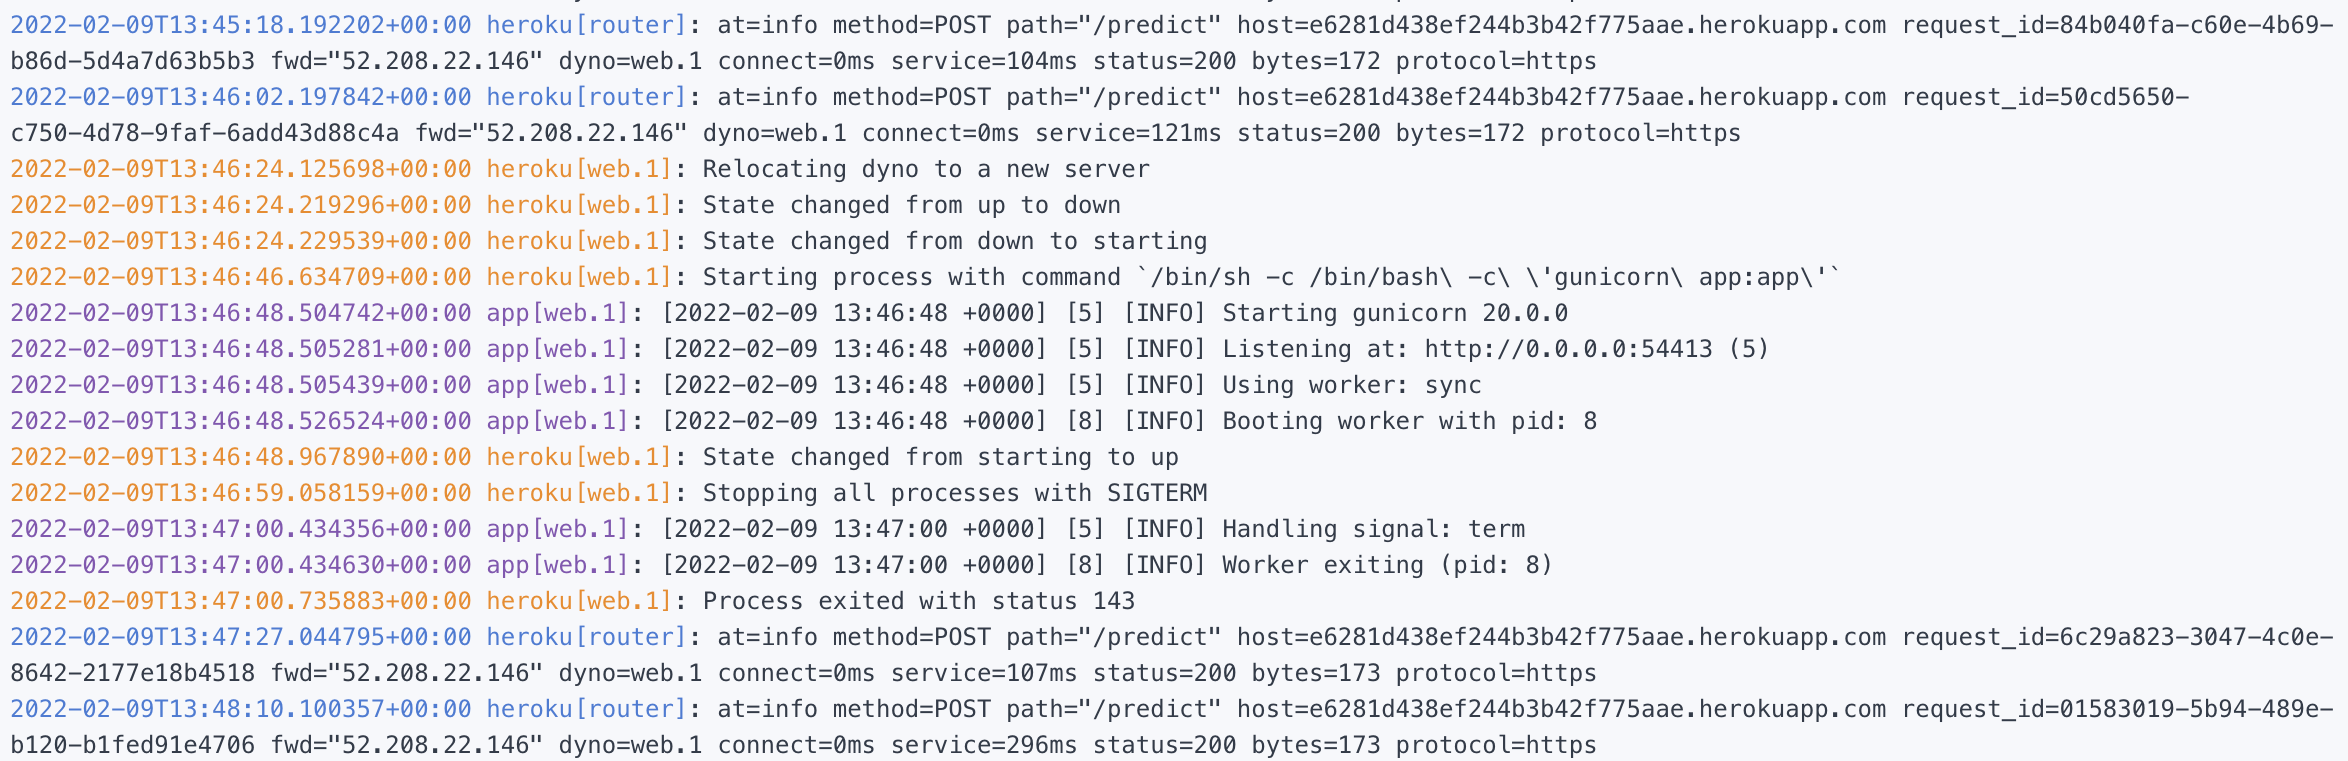
\includegraphics[width=1\textwidth]{images/log_screenshot.png}
	\caption{Logs of heroku dyno relocation to a new server}
	\label{fig:heroku_relocating}
\end{figure}

This issue does not seem to have impacted the application, however one can note that it took \SI{1}{\minute} and \SI{30}{\second} to complete the whole application relocation. Knowing the rate of requests was roughly one per minute, it is possible that some data was lost in the process.

This issue was imposed by the \texttt{heroku} platform, and as highlighted on the first report this kind of issues were out of the Awkward Problem Solutions™ control. 

Other than that, no unexpected error occurred during the whole week in production.

\subsection{Learnings and Future Improvements}

The application deployment was perhaps the part of the current project that was better executed. Some of the key takeaways that revealed important are related to the overall app's robustness.

First of all, it is highly important to develop a broad model pipeline capable of receiving all types of data, specially \texttt{NaN}, and still output a result.

Then, the app itself has to be able to interpret the data that the REST API user provides. During this project an effort was made to interpret the data, discarding requests only as the last resort.
For instance, when a field type is an integer, but the REST API user provides the string \textit{"11"} the app should be able to convert into the number $11$, without discarding the request as invalid.
Relying on the database to do this kind of heavy lifting was an important learning from this project. Since the database is, by definition, able to do this type of conversions leveraging this functionality improved the app robustness and increased the development speed.

Moreover, an important feature that was overlooked during the preparation for the production week is access to logs. This was a known limitation from \texttt{heroku}, but the information it provides is highly valuable and should never be missed in a production application. 

Given the limitation, one alternative would be adding a second table with the triggered exceptions. However, this alternative was not viable for the current project, since it imposed a data loss risk due to the \SI{10000}{rows} limitation from \texttt{heroku}. A different alternative would be creating a local log file to be accessed later.

Finally, \texttt{DBeaver} revealed to be an important tool during the deployment and production stage. It allowed accessing the remote database hosted by \texttt{heroku} and proved to be a valuable monitoring tool. On top of that, it made the extraction of the database into a \texttt{csv} file seamless and quick.

% Store all log messages, store all requests (?)








\end{document}
